\documentclass[border=10pt]{standalone}

\usepackage{tikz}
\usepackage{tikzsymbols}
\usetikzlibrary{calc,patterns,shapes.geometric}

\def\centerarc[#1](#2)(#3:#4:#5){\draw[#1] ($(#2)+({#5*cos(#3)},{#5*sin(#3)})$) arc (#3:#4:#5);}

\begin{document}
	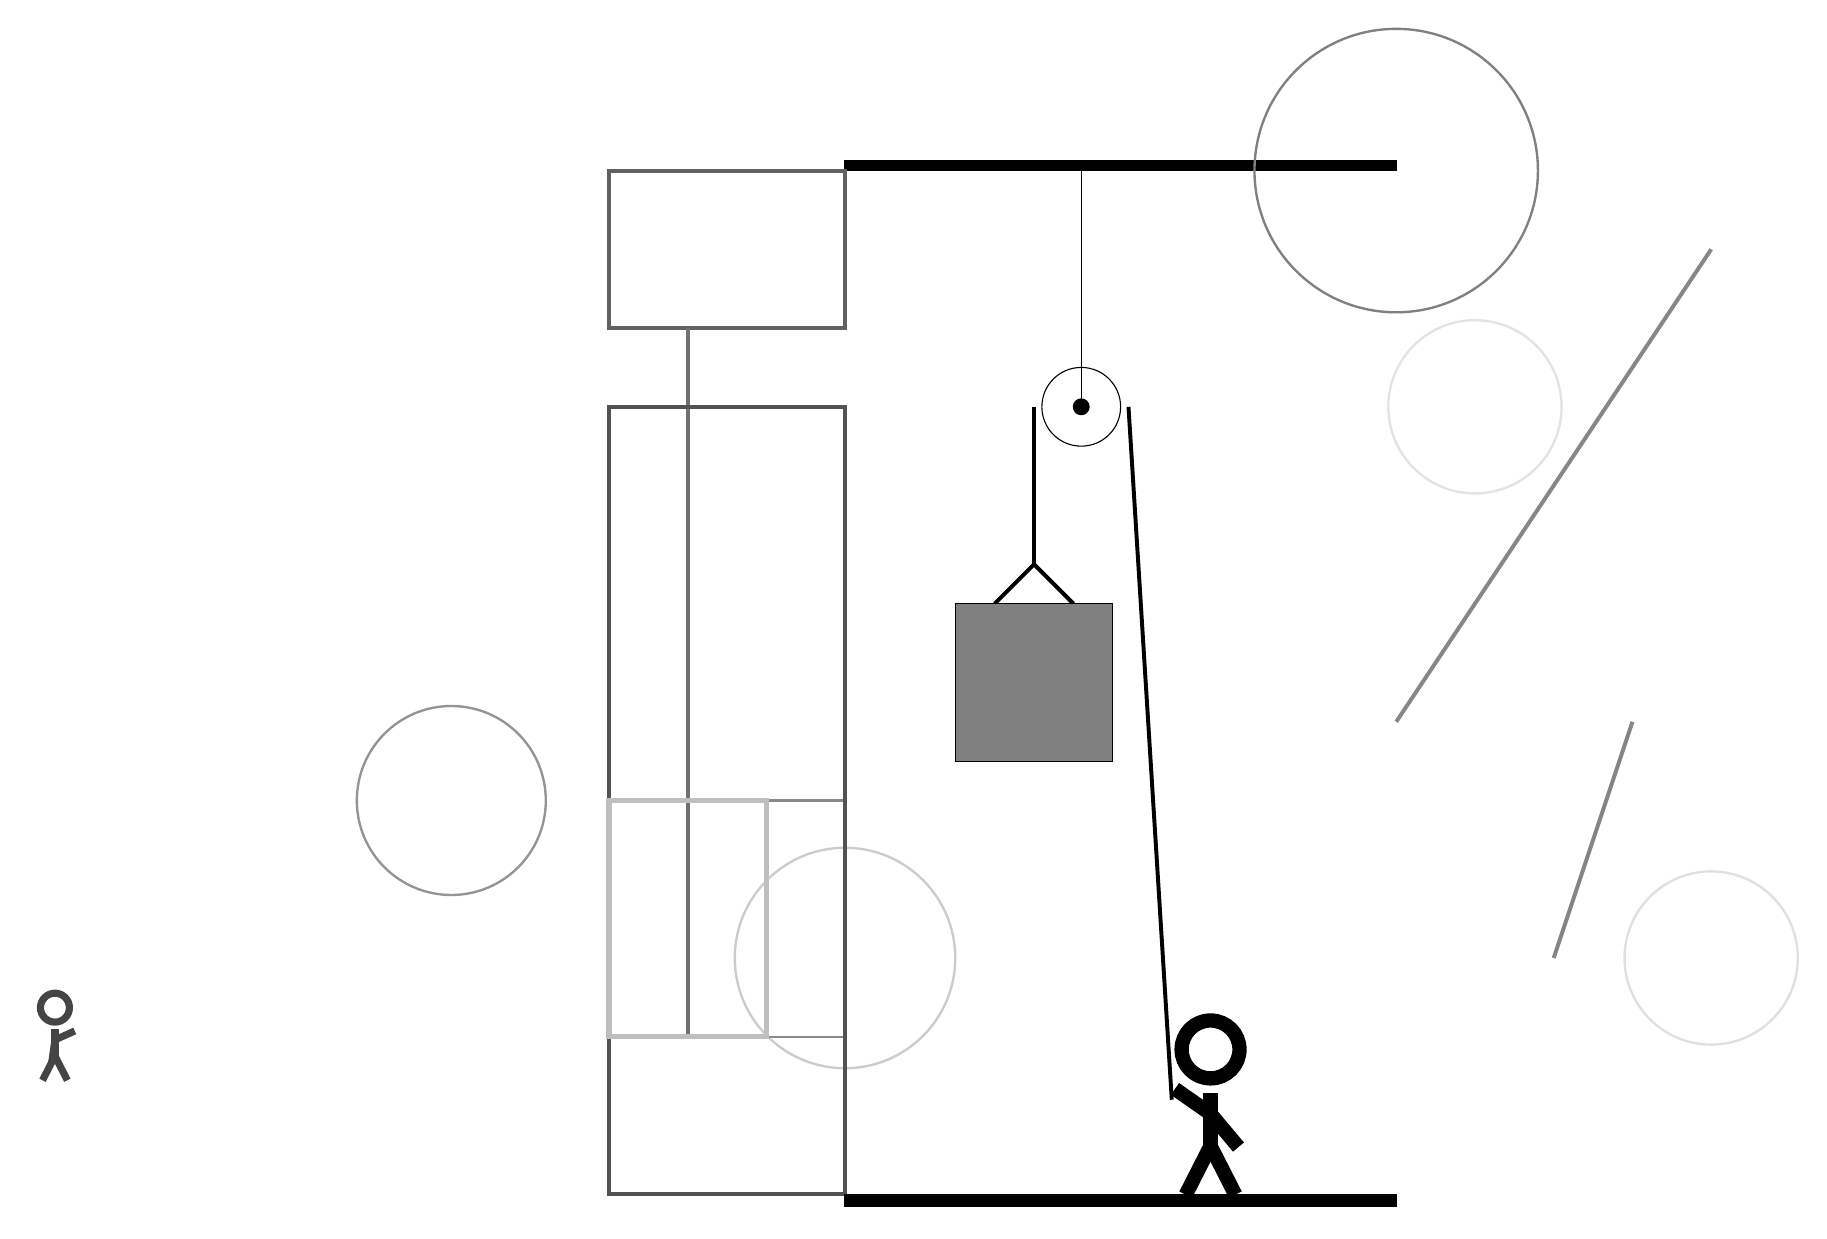
\begin{tikzpicture}
		%%%%% START %%%%%
		
		\draw[fill=black] (-2, 10) rectangle (5, 10.125);
		
		\draw (1, 7) circle (0.5);
		\draw[fill=black] (1, 7) circle (0.1);
		\draw (1, 10) -- (1, 7);
		
		\draw[line width=0.5mm] (-0.1, 4.5) -- (0.4, 5.0) -- (0.9, 4.5);
		\draw[fill=black!50] (-0.6, 4.5) rectangle (1.4, 2.5);
		
		\draw[line width=0.5mm] (0.4, 7) -- (0.4, 5.0);
		\centerarc[line width=0.5mm](1, 7)(0:180:0.6);
		\draw[line width=0.5mm](1.6, 7) -- (2.15, -1.8);
		
		\node at (2.6, -1.9) {\Strichmaxerl[10][-35][-50]};
		
		\draw [line width=0.3mm, color=black!20](-2, 0) circle (1.4);
		
		\draw[line width=0.5mm, color=black!62] (-2, 8) rectangle (-5, 10);
		\draw[line width=0.3mm, color=black!46] (-2, 2) rectangle (-4, -1);
		\draw [line width=0.3mm, color=black!11](6, 7) circle (1.1);
		\draw[line width=0.5mm, color=black!47](9, 9) -- (5, 3);
		\draw [line width=0.3mm, color=black!42](-7, 2) circle (1.2);
		
		\node[line width=0.3mm, color=black!73] at (-12, -1) {\Strichmaxerl[5][82][24]};
		
		\draw[line width=0.5mm, color=black!56](-4, -1) -- (-4, 8);
		\draw[line width=0.5mm, color=black!48](7, 0) -- (8, 3);
		
		\draw[line width=0.5mm, color=black!68] (-2, -3) rectangle (-5, 7);
		
		\draw [line width=0.3mm, color=black!12](9, 0) circle (1.1);
		\draw [line width=0.3mm, color=black!28](-6, 6) circle (0.0);
		\draw[line width=0.7mm, color=black!25] (-3, 2) rectangle (-5, -1);
		
		\draw [line width=0.3mm, color=black!50](5, 10) circle (1.8);
		
		\draw[fill=black] (-2, -3) rectangle (5, -3.15);
		
		%%%%% END %%%%%
	\end{tikzpicture}
\end{document}